%\documentclass[varwidth]{standalone}
\documentclass[10pt]{amsart}
\usepackage{amscd,amsxtra,color,amsthm}

\usepackage[all]{xy}
\usepackage{etex}
\usepackage{pictex}
\usepackage{graphicx}
\usepackage{tikz}
\usepackage[utf8]{inputenc} 
\usepackage[T1]{fontenc}
\usepackage[all]{xy}
\usepackage{etex}
\usepackage{pictex}
\usepackage{graphicx}
\usepackage{mathtools}
\DeclarePairedDelimiter{\ceil}{\lceil}{\rceil}
\DeclarePairedDelimiter{\floor}{\lfloor}{\rfloor}
\usepackage{comment}
\usepackage{changepage}


\textheight=9in \textwidth=6.2in \topmargin=0in
\oddsidemargin=.15in \evensidemargin=.15in

\begin{document}
\parskip10pt
\parindent12pt
\baselineskip16pt





%%%%%%%%%%%%%%%%%%%%%%%%%%%%%%%%%%%%%%%%%%%%%%%%%%%%%%%%%%%%%%%%%%%%%%%%%%%%%%%%%%%%%%%%%%%%%%%%
%%  Definitions
%%%%%%%%%%%%%%%%%%%%%%%%%%%%%%%%%%%%%%%%%%%%%%%%%%%%%%%%%%%%%%%%%%%%%%%%%%%%%%%%%%%%%%%%%%%%%%%%

\def\G{\widetilde{G}}
\def\B{\widetilde{B}}
\def\T{\widetilde{T}}
\def\C{\mathbb{C}}
\def\A{\mathbb{A}}
\def\Z{\mathbb{Z}}
\def\R{\mathbb{R}}
\def\Q{\mathbb{Q}}
\def\N{\mathbb{N}}
\def\C{\mathbb{C}}
\def\F{\mathbb{F}}
\def\I{\mathbb{I}}
\def\H{\mathcal{H}}
\def\e{\varepsilon}
\def\s{\underline s}
\def\z{\zeta }
\def\vp{\varpi }
\def\O{\mathcal O}
\def\v{\upsilon }
\def\U{\Upsilon }
\def\p{\wp }
\def\p{\mathfrak{p}}
\def\B{\mathfrak{B}}

\newtheorem{theorem}{Theorem}%[section]
\newtheorem{lemma}[theorem]{Lemma}


\title{Proof for Closed Eulerian Trails}

\author{Graham Swain}
%\centerline{Your name goes here.}




\begin{abstract}
In this paper we explore a proof showing that a graph contains a closed Eulerian trail if and only if
all of its vertices have even degree. We show part of this proof by developing an algorithm.
\end{abstract}

\maketitle



%\begin{abstract}
%abstract goes here....
%\end{abstract}

%\maketitle

\section{Introduction}

This problem dates back to 18th century K\"{o}nigsberg, Prussia, modern day Kaliningrad, Russia. 
K\"{o}nigsberg had seven bridges that connected four landmasses, the figure below shows roughly 
how the bridges were arranged. The citizens of K\"{o}nigsberg wonder if a person could walk across 
town and cross each bridge exactly once.

\begin{figure}[h!]
\centerline{
{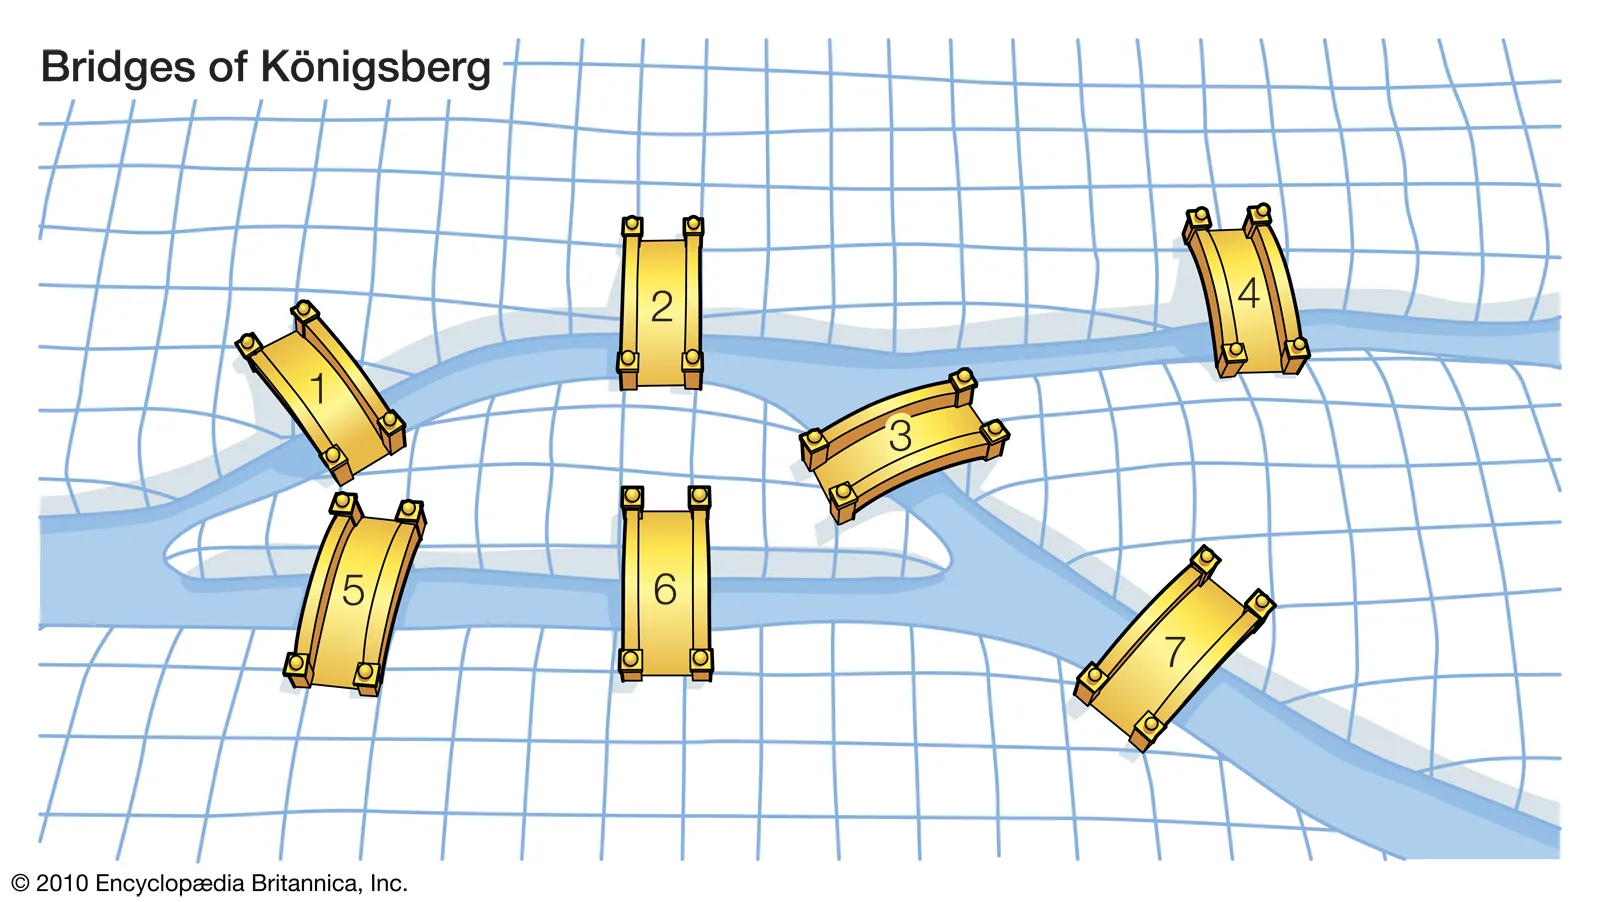
\includegraphics[width=.7\textwidth]{pictures/bridge_pic.png}}}\label{bridge}
\end{figure} 

The problem was solved by Leonard Euler, who found it to be impossible. His reasoning was that 
every time you enter a landmass you must also be able to leave it, so any landmass with and odd
number of bridges coming from it would cause you to get stuck. There is an exception for the landmass
that you start and end on, but in K\"{o}nigsberg each landmass has an odd number of bridges coming from
them. This led to the theorem we are looking at today as well as set the basis for graph theory.

\section{Definitions}
\noindent
Before we look at the theorem, we first must go over some definitions to help understand it.

\noindent
\textbf{Definition} 
\emph{
    A \textbf{graph} G = (V,E) is comprised of a set of vertices V and a set of 
    different undordered pairs of distinct vertices from V. Elements from E are called edges.
}

\noindent
\textbf{Definition} 
\emph{
    Two vertices v, w that exist in V are said to be \textbf{adjacent} if the
    edge vw exits in E.
}

\noindent
\textbf{Definition}
\emph{
    If ab exits in E, then we say that the vertex v and the edge vw are \textbf{incident}; w would
    also be incident with vw.
}

\noindent
\textbf{Definition}
\emph{
    The \textbf{degree} of a vertex v that exits in V is the amount of edges in E that are incident
    with v.
}

\noindent
\textbf{Definition}
\emph{
    A \textbf{walk} W is a finitie sequence of vertices in which each consecutive pair of vertices
    are adjacent.
}
Vertices and edges are allowed to be repeated in a walk, with the exception of the same vertex consecutively.

\noindent
\textbf{Definition}
\emph{
    A \textbf{trail} T is a walk in which edges are not allowed to be repeated. A trail is called a 
    \textbf{closed trail} when the trail begins and ends at the same vertex.
}

\noindent
\textbf{Definition}
\emph{
    A trail that contains all of the edges in E is called an \textbf{Eulerian trail}. A \textbf{closed
    Eulerian trail} when the trail begins and ends at the same vertex.
}

\noindent
\textbf{Definition}
\emph{
    A graph is said to be \textbf{connected} if, and only if, there is a walk between any two vertices
    v and w.
}

\section{Theorem and Proof}

\begin{theorem} \ 
    A connected graph has a closed Eulerian trail if and only if all of its vertices have even degree.
    \label{theorem1}
\end{theorem}

\begin{proof} 
    ($\Rightarrow$) Assume a connected graph $G$ has a closed Eulerian trail, denoted as $C$. Prove that
    every vertex has an even degree. 
    
    \noindent
    Take an arbitrary vertex $v$. As we traverse $C$, each time we enter $v$ we must be able to exit on a
    distinct edge. Thus every vertex must be incident with 2$k$ edges, where $k$ is the number of times
    a vertex is visited. Therefore every vertex has an even degree. 

    \noindent
    The first vertex of $C$ does make a special case. It does not matter since we chose an arbitrary
    vertex in the first step, but we can still look at it. Denote the first vertex of $C$ as $a$. We
    know that $a$ is incident to the first edge of $C$, the last edge of $C$, as well as a 2$k$ amount
    of other edges. So $a$ is adjacent to \\
    \centerline{$1+2k+1 = 2+2k$} \\
    edges, which will result in an even number.

    \noindent
    ($\Leftarrow$) Assume $G$ is a connected graph with every vertex having even degree. Prove that
    it has a closed Eulerian trail.

    \noindent
    To prove this direction we must construct an algorithm. 
    
    \noindent
    \textbf{Step 1.} Pick an arbitrary vertex $v$ to act as our starting point.

    \noindent
    \textbf{Step 2.} Construct a trail beginning at $v$. Continue to add edges to this trail until we
    arrive back at $v$. (\emph{We know we arrived at $v$ since if we entered another vertex $a$ that we
    could not leave then $a$ has an edge to enter on but not a corresponding edge to exit on. Which would
    mean that $a$ has an odd degree, which would be a contradiction.}) Since we did arrive back at
    $v$ we formed a closed trail, which we will called $C_1$.

    \noindent
    \textbf{Step 3.} Check if $C_1$ contains all the edges of $G$. If it does we have found a closed
    Eulerian trail and are done. If it does not contain all of the edges of $G$ then we continue to
    \textbf{Step 4}.

    \noindent
    \textbf{Step 4.} Remove all of the edges in $C_1$ from $G$. We will call the resulting graph $G'$.
    $G'$ does not need to be connected.

    \noindent
    \textbf{Step 5.} Choose an arbitrary vertex $w$ that is in both $C_1$ and $G$.

    \noindent
    \textbf{Step 6.} Construct a trail in $G'$ beginning at $w$ and continue until we arrive back at
    $w$. We will call the resulting closed trail $C_2$.

    \noindent
    \textbf{Step 7.} Combine $C_1$ and $C_2$ to form a new closed trail denoted as $C'$. If $C'$
    contains all of the edges of $G$, we have found a closed Eulerian trail and are done. If not 
    continue to \textbf{Step 8.}

    \noindent \emph{
        We know that combining two closed trails form a new closed trail. To show this, start at $v$
        in $C_1$. Trace $C_1$ until we arrive at $w$. Once we reach $w$, trace the entirity of $C_2$.
        Once we arrive back at $w$, continue tracing $C_1$ until we end at $v$. The trace is $C'$.
    }

    \noindent
    \textbf{Step 8.} Remove all of the edges of $C'$ from $G$ to get $G''$. Chose a vertex in both
    $C'$ and $G''$ and continue in this manner until we have removed all the edges of $G$.

    
\end{proof}

In the tex file, note that a label was added within the above theorem environment.  This is so that you can refer to Theorem \ref{theorem1} and if you add more theorems to the paper, they will automatically be renumbered.  The same is true for references.  You may refer to \cite{R}.  It may be necessary to compile the tex file twice before the labels show up.  All sources used in your paper should be listed as in the samples below.  The first, second, and fifth references are articles, while the third and fourth are books.

Here is a sample of a math environment: $\sqrt[4]{14}$.  Use double $\$$ if you wish to have a math environment centered on a line by itself:
$$\mathop{\int}\limits_{1}^{\infty} e^{-x} \ dx.$$
If you would like to have an equation be numbered, use the following:
\begin{equation}  4x^5+3y^7=85. \label{eq} \end{equation}
You can then refer label in the equation.  Eg., equation (\ref{eq}) pulls up the correct number.

Equations, inequalities, etc... can be aligned using the following commands:
\begin{align} \delta (H) &= n-(r-1)-\Delta (\overline{H}) \notag \\
                                    &\ge n-(r-1)-(m+2) \notag \\
                                    &\ge n-m-r-1 \label{ineq} \end{align}
As with the equation environment, each line that has $\backslash$notag will not be labelled, and putting a label allows you to refer to property (\ref{ineq}).

Matrices can be created using the array command:

$$\left( \begin{array}{rrr} -2 & 3 & -7 \\ 2 & 0 & 4 \end{array} \right)$$
% Note that the 3 r's after the above array command right-align the entries.  Replacing any of them with l or c will left-align or center the corresponding columns.

\bibliographystyle{amsplain}
\begin{thebibliography}{10}

\bibitem{C} V. Chv\'atal, {\it Tree-complete Graph Ramsey Numbers,}  J. Graph Theory {\bf 1} (1977), 93.

\bibitem{CH} V. Chv\'atal and F. Harary, {\it Generalized Ramsey Theory for Graphs III. Small Off-diagonal Numbers,} Pacific J. Math. {\bf 41} (1972), 335-345.

\bibitem{IR} K. Ireland and M. Rosen, ``A Classical
Introduction to Modern Number Theory,'' $2^{nd}$ edition,
Springer-Verlag, 1990.

\bibitem{J} G. Janusz, ``Algebraic Number Fields,'' $2^{nd}$ edition, Graduate Studies in Mathematics {\bf 7}, American Mathematical Society, Providence, RI, 1996.

\bibitem{R} F. Ramsey, {\it On a Problem of Formal Logic,} Proc. London Math. Soc. {\bf 30} (1930), 264-286.



\end{thebibliography}


\end{document}
